\documentclass{standalone}
%<--------------------------------------------------------------------------->%
%%% TikZ %%%
\usepackage{tikz}
% \usetikzlibrary{calc}
% \usetikzlibrary{angles,quotes}
% \usetikzlibrary{intersections,topaths}
% \usetikzlibrary{decorations.markings}
%<--------------------------------------------------------------------------->%

\begin{document}

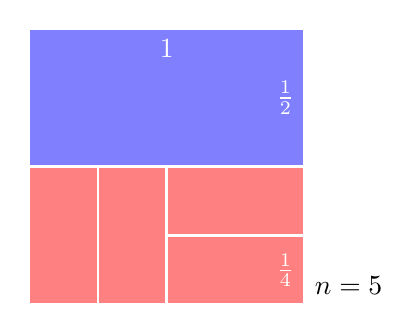
\begin{tikzpicture}[scale=3.5,thick,line cap=round,rotate=90]
	\tikzstyle{jiao}=[solid,circle,draw,fill=white,inner sep=.8pt];
	\tikzstyle{tile1}=[line width=0.1em,draw=white,fill=blue!50];
\tikzstyle{tile2}=[line width=0.1em,draw=white,fill=red!50];
\tikzstyle{tile3}=[line width=0.1em,draw=white,fill=blue!50!red!60];
\tikzstyle{tile4}=[line width=0.1em,draw=white,fill=blue!20!red!60];

	\draw[tile1] (1/2,0) rectangle (1,1);
	\draw[tile2] (0,0)   rectangle (1/4,1/2);
	\draw[tile2] (1/4,0) rectangle (1/2,1/2);
	\draw[tile2] (0,2/4) rectangle (1/2,3/4);
	\draw[tile2] (0,3/4) rectangle (1/2,1);
	% \draw[dotted,draw=black,opacity=0.4] (0,0) rectangle (1/2,1);
	% \draw[dotted,draw=black,opacity=0.4] (0,1/2) -- (1/2,1/2);
	\node[white,left]  at (1/8,0) {$\frac{1}{4}$};
	\node[white,left]  at (3/4,0) {$\frac{1}{2}$};
	\node[white,below] at (1,1/2) {$1$};
	\node[above right] at (0,0) {$n=5$};
\end{tikzpicture}

\end{document}
